% !TeX root = ../Doc_especific_mse_anchovy.tex

\begin{figure}[H]
    \centering
    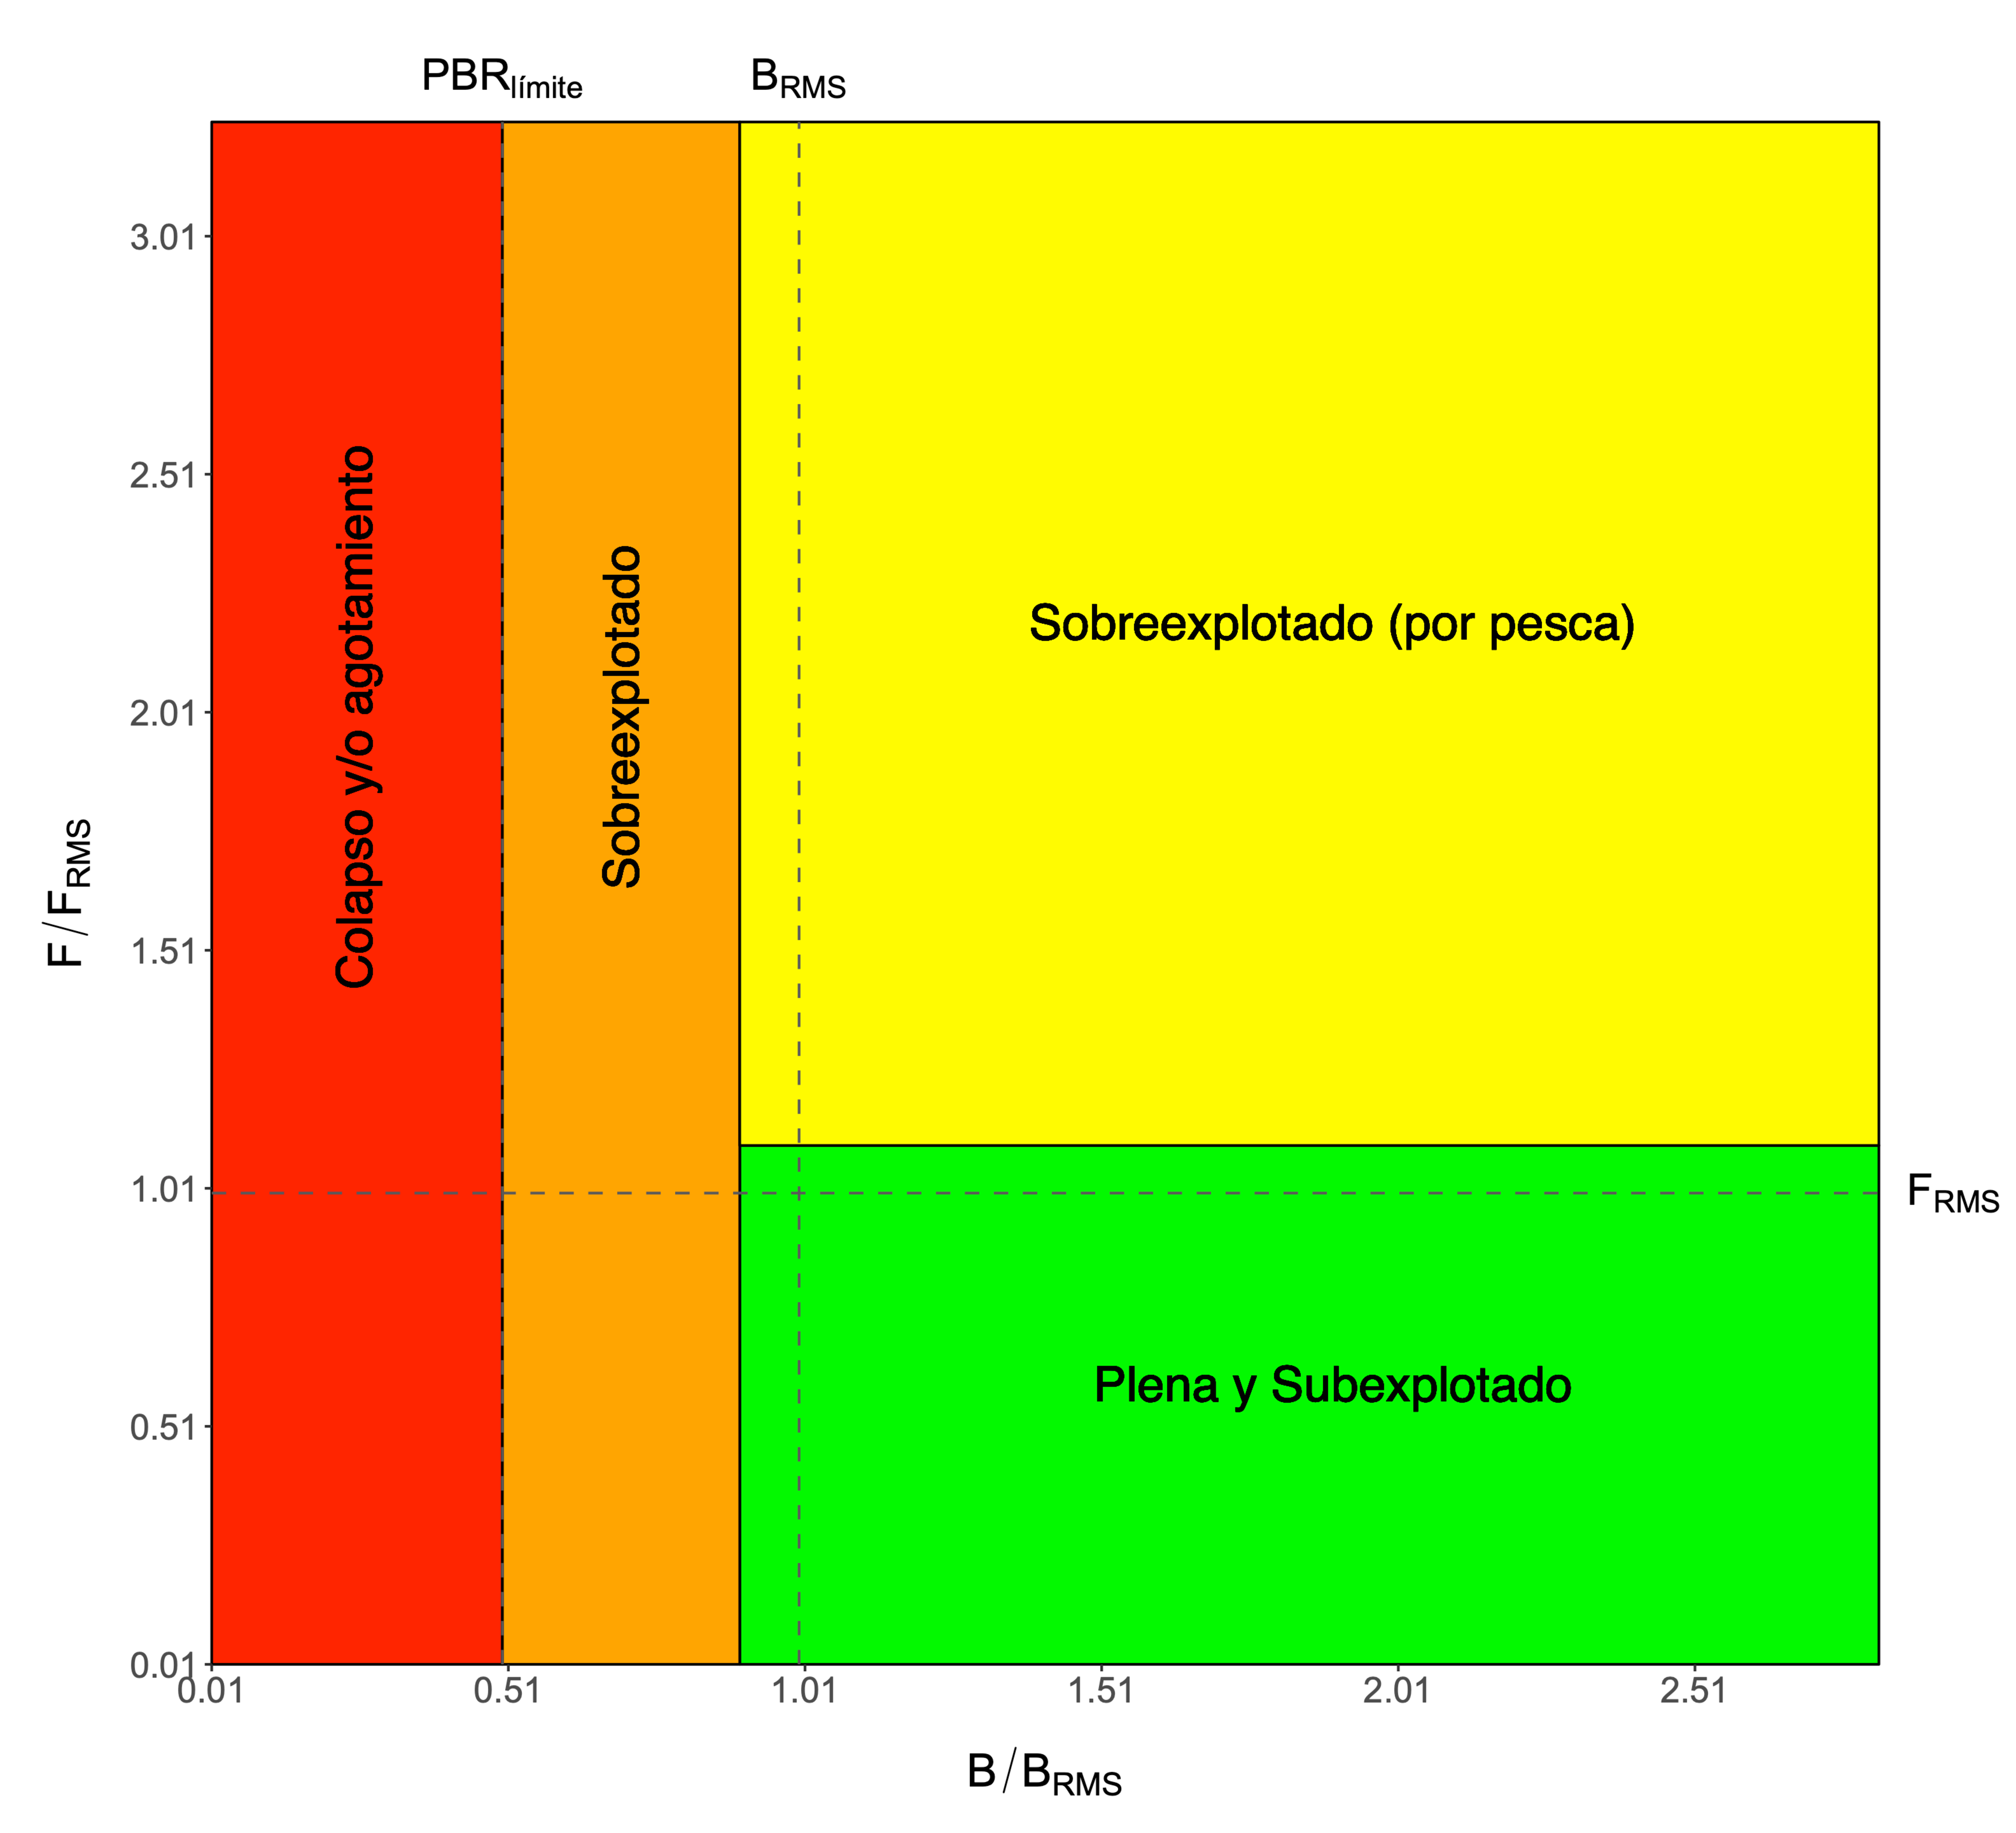
\includegraphics[scale=0.1]{figura6.pdf}
    \caption{Diagrama de fase tipo para la pesquería de recursos pequeños pelágicos, acordados por el CCT y el grupo de trabajo del taller openMSE. Según la SUBPESCA la zona verde corresponde a la región deseada para el manejo pesquero.}
    \label{fig:figure6}
\end{figure}

\begin{figure}[H]
    \centering
    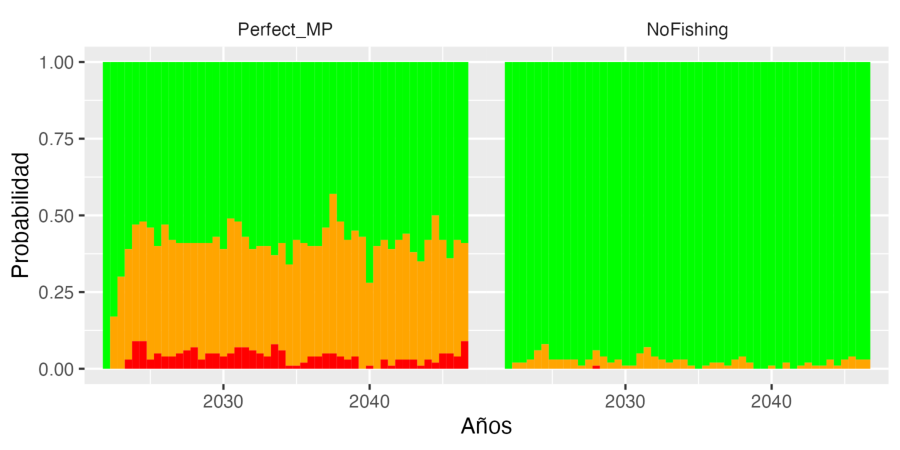
\includegraphics[scale=1]{figura7.pdf}
    \caption{Diagrama de fase temporal (Kobe time plot), con la proporción de las simulaciones de la condición del stock de anchoveta para cada año de la proyección, para dos procedimientos de manejo (Conocimiento perfecto y Sin capturas).}
    \label{fig:figure7}
\end{figure}

\begin{figure}[H]
    \centering
    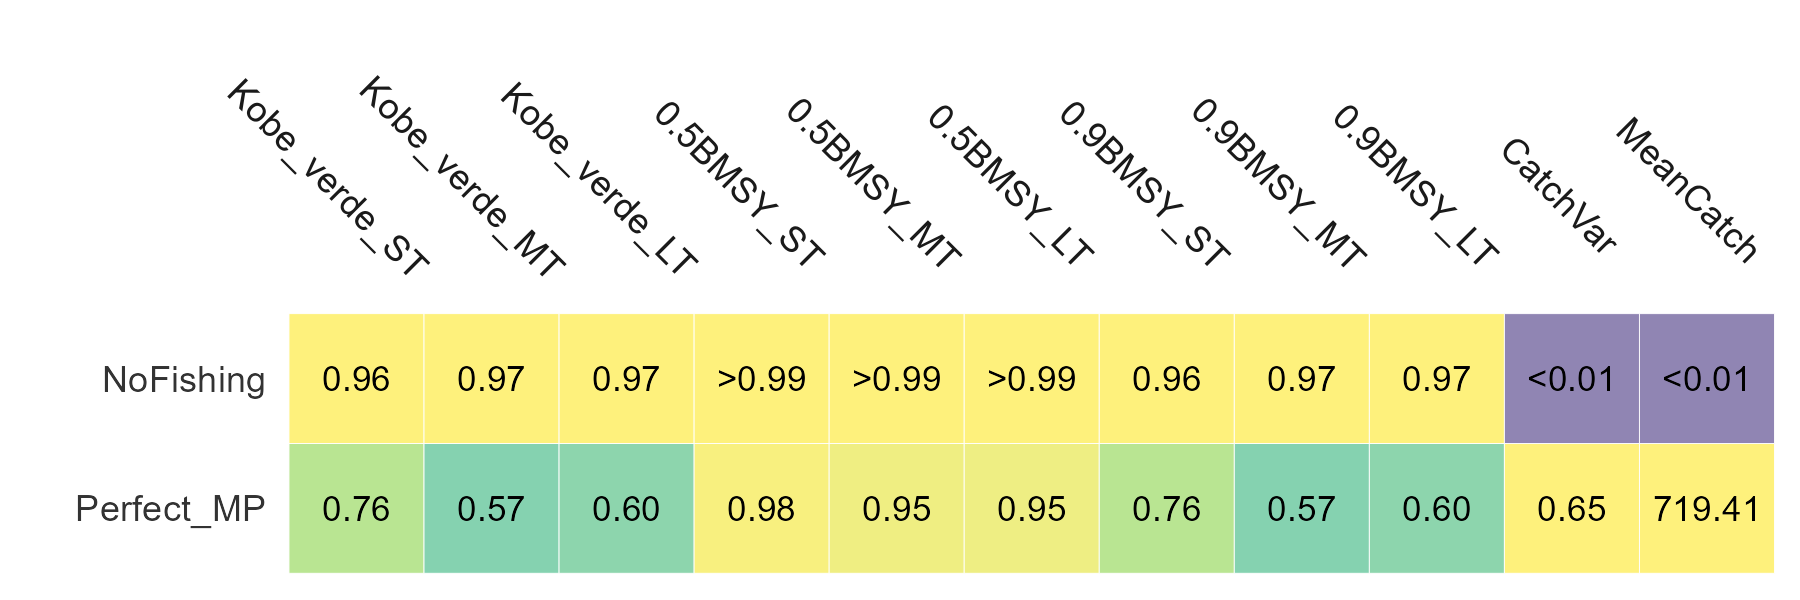
\includegraphics[scale=0.32]{figura8.png}
    \caption{Niveles de probabilidad asociados a los procedimientos de manejo y medidas de desempeño para los ejercicios evaluados durante el transcurso del taller.}
    \label{fig:figura8}
\end{figure}